%!TEX root = ../article.tex

% Implementation
\section{Implementation}
\label{sec:implementation}
This section describes the implementation details for the solution proposed in Section~\ref{sec:solution}.
Here we describe the implementation and technological details for the provisioning mechanism. Also, we
describe the technological components of our smart warehouse for the deployment approaches based in
the cloud and fog concepts.

% Smart Warehouse Deployment
\subsection{Smart Warehouse Deployment}
\label{sub:impl_smart_place}
The smart warehouse setup was based in a demonstration scenario described by Correia et al. \cite{correiaalpharfid}.
The warehouse is composed of a robot transporting tagged products that are identified by \gls{RFID} readers
deployed in the physical space. To monitoring the robot inside the warehouse, we decide to use Fosstrak
as our \gls{RFID} middleware. In our implementation, the \gls{RFID} readers are emulated through the
Rifidi Emulator, which uses the \gls{LLRP} protocol to communicate with the Fosstrak platform.

% Cloud approach
\subsection{Cloud Deployment}
\label{sub:imp_smart_warehouse_cloud}

The \gls{RFID} middleware is provisioned in the cloud in a single virtual machine. In the
Fosstrak implementation the \gls{FCServer}, \gls{EPCIS} repository and the Capture application
requires an Apache servlet container to deploy and run the web applications. The \gls{EPCIS}
repository is connected to a MySQL database that stores the event data. The smart warehouse can be
connected to the cloud through a physical (e.g. \gls{ADSL} or Fiber-optic) to a wireless
connection (e.g. Wi-Fi, 3G or \gls{LTE}).

% Fog approach
\subsection{Fog Deployment}
\label{sub:imp_smart_warehouse_fog}
The \gls{RFID} middleware is provisioned across the fog and the cloud. At the cloud,
all the software components are provisioned in a single \gls{VM}. The \gls{EPCIS} repository is deployed
and running on top of an Apache Tomcat servlet instance. The repository is connected to a MySQL
database, which stores the event data. In the current implementation the fog was built with a traditional
\gls{VM}. The \gls{FCServer} and the Capture application are deployed and running on top of a single
Tomcat servlet instance. The Capture application sent the events collected by the \gls{FCServer} to
the \gls{EPCIS} repository through the \textit{\gls{EPCIS} Capture Interface} - via \gls{HTTP} requests.
Both the smart warehouse as the fog can be connected respectively to the fog and cloud through several
types of connection, from a physical connection (e.g. \gls{ADSL} or Fiber-optic) to a wireless connection
(e.g. Wi-Fi, 3G or \gls{LTE}).

% Smart Place Provisioning
\subsection{Smart Place Provisioning}
\label{sec:impl_provisioning}
The implementation of the provisioning mechanism relies on the Chef\footnote{The tool uses culinary
analogy in most of its concepts} tool. Chef provides several features that allows to describe our
infrastructure as code. In the implementation of the provisioning mechanism, the main features used
were the Chef \textit{recipes}, \textit{roles} and the \textit{knife} command-line tool.\\

In order to provisioning the smart place software stack, we defined a set of recipes and roles that
are used by Chef to provisioning the application infrastructure. These recipes describe how the
Fosstrak software stack is provisioned in the cloud - since we are using Docker containers to
provisioning Fosstrak stack, the recipes describe how to provisioning the Docker containers -
and the roles allow to specify which recipes must be applied to a given node as well to
attribute responsibilities to a specific node in the provisioned infrastructure.

% Provisioning Mechanism
\subsection{Provisioning Mechanism}
\label{subs:provisioning_mechanism}
To provisioning the resources in the cloud instances we will use \textit{knife}, a command-line tool
developed by Chef that provides an interface between the local Chef repository and the Chef server.
The provisioning workflow is illustrated in Figure~\ref{fig:provisioning_tech_architecture}.\\

% Automatic provisioning diagram
\begin{figure}[ht!]
  \centering
  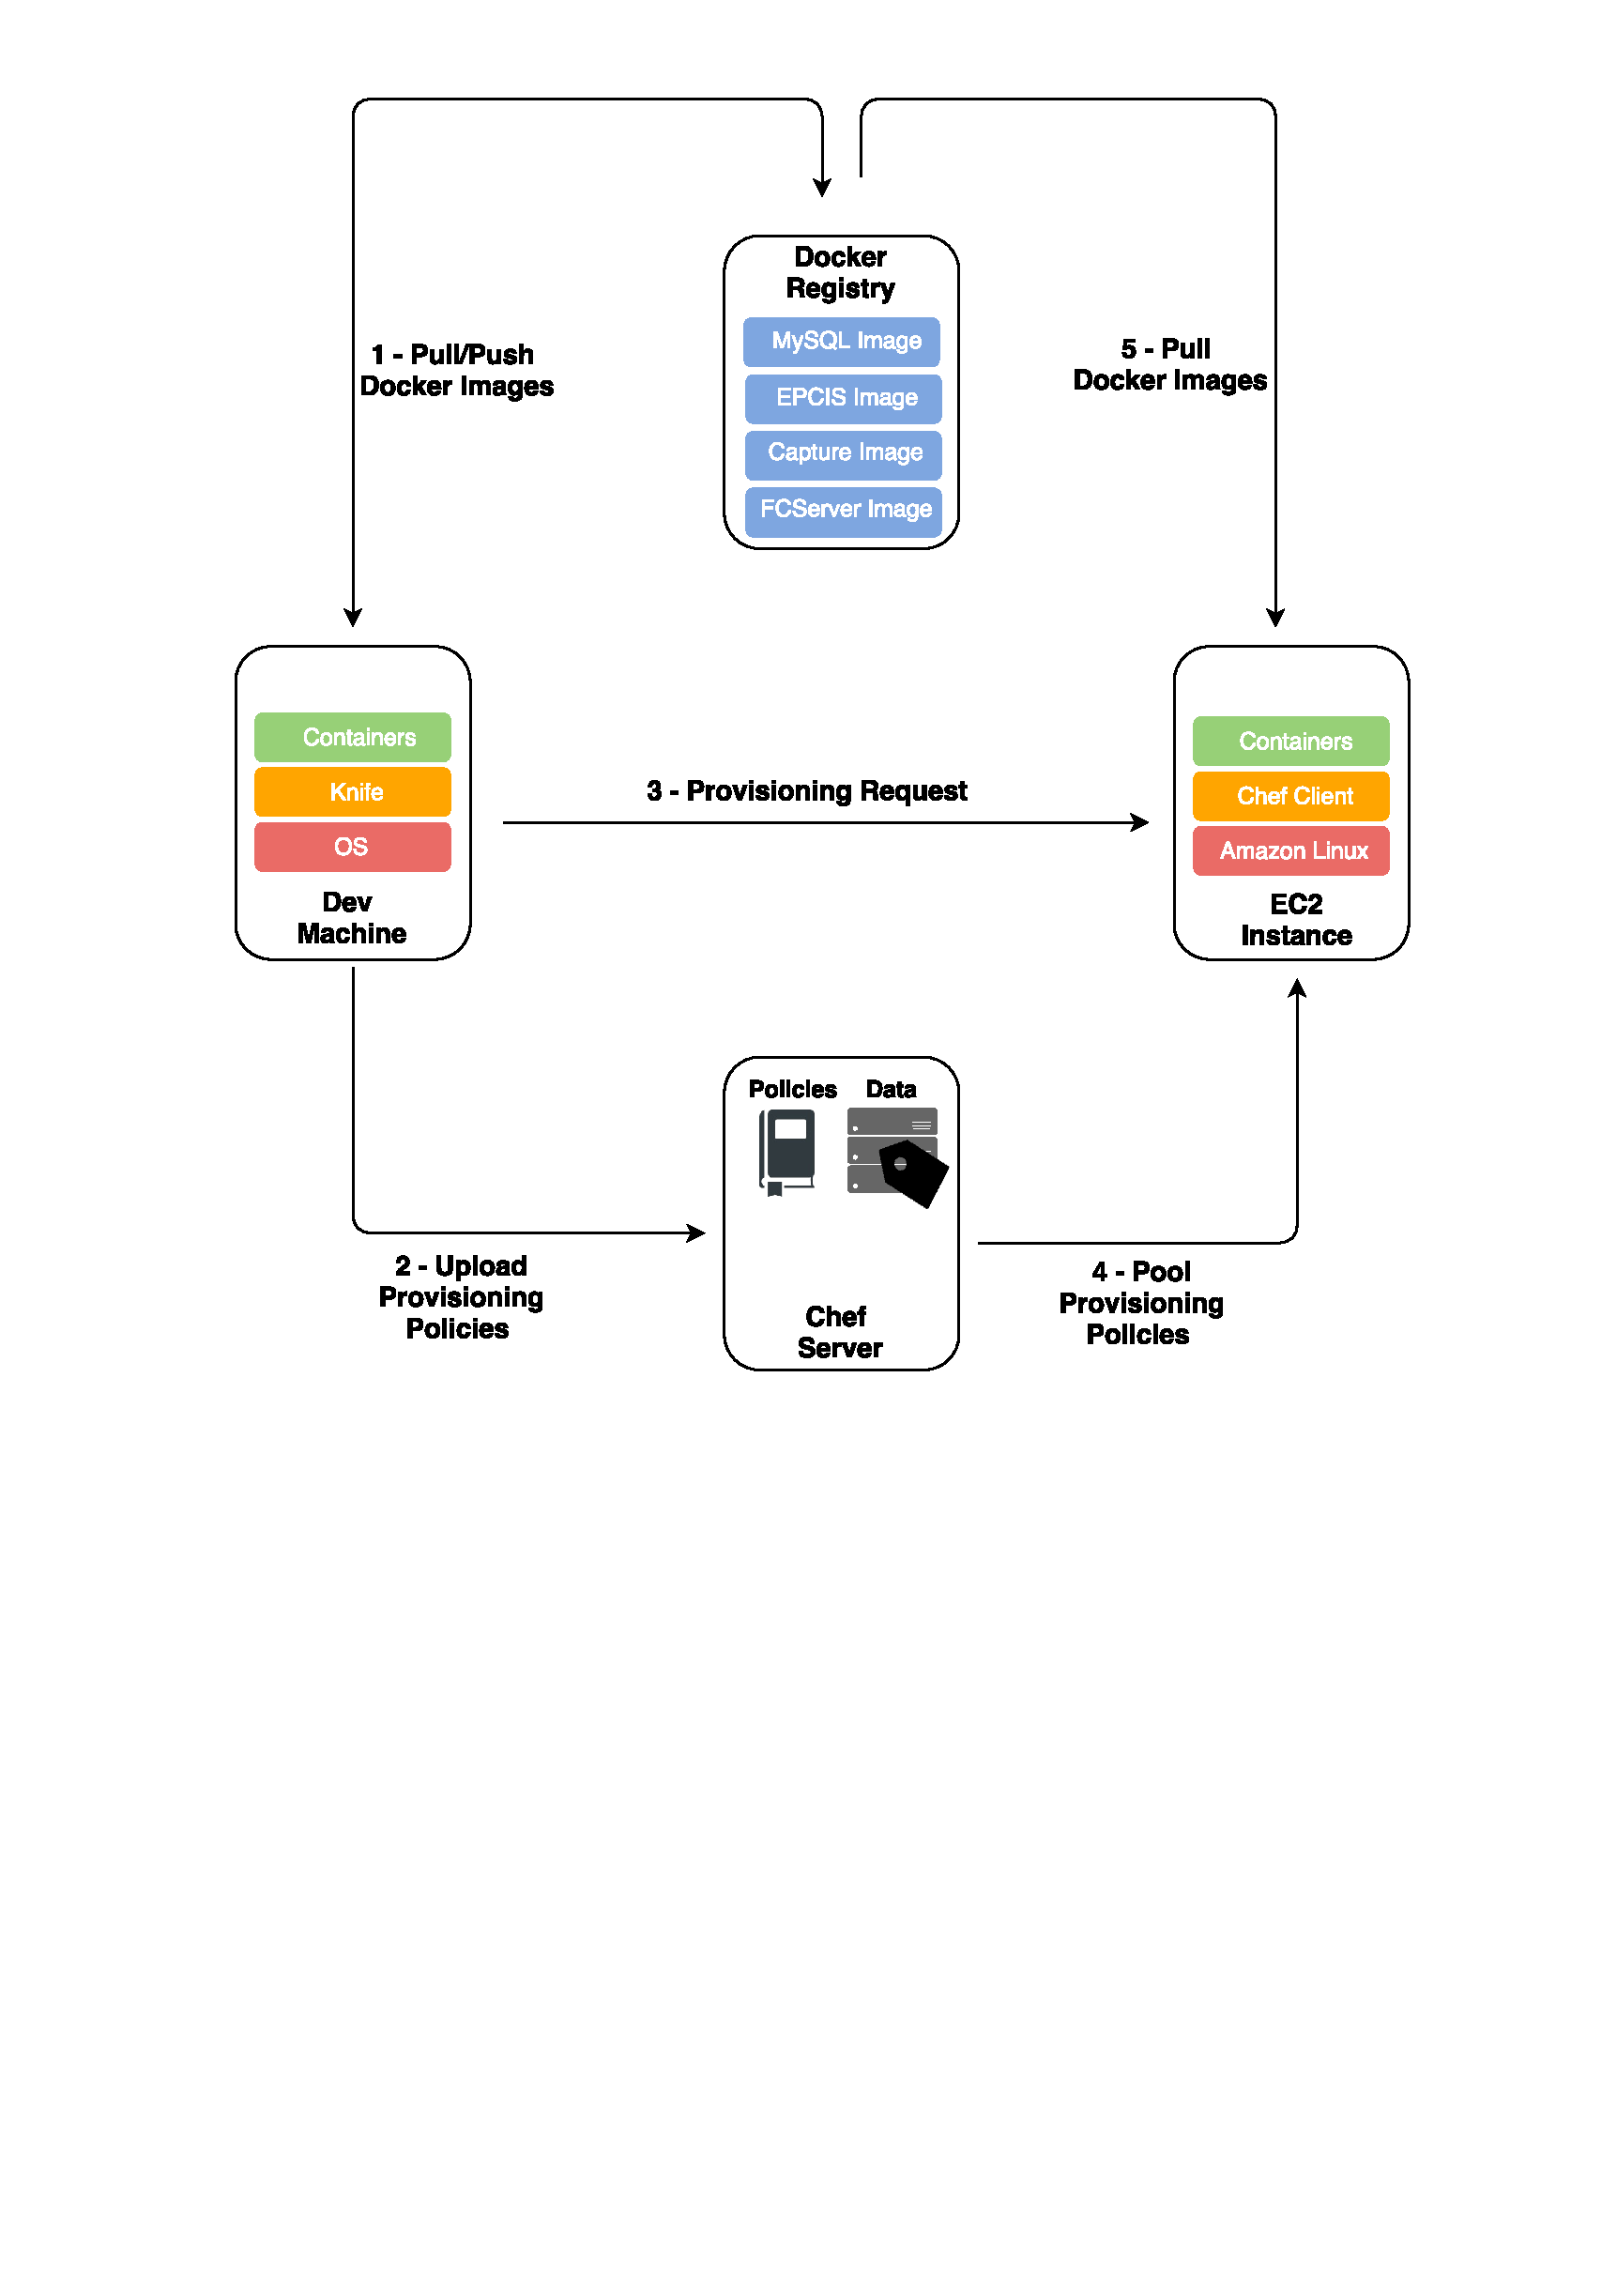
\includegraphics[width=.5\textwidth]{./figures/c4t-tech-architecture}
  \caption[Automatic provisioning workflow.]{Automatic provisioning workflow.}
  \label{fig:provisioning_tech_architecture}
\end{figure}

In a development environment the Docker images are built and then uploaded to the Docker Registry
repository (1). The provisioning of the cloud resources is described in the cookbooks that are uploaded
to the Chef server (2). The provisioning request (3) is performed using \textit{knife}, that allows to
describe the image type, the instance type and the policies - e.g. the \textit{role(s)} and/or \textit{recipe(s)} -
that need to be applied on each provisioned node. Then the Chef client runs the configuration policies
that are pulled from the Chef server (4). In our solution the Chef client apply the configuration recipes
that are described in the role assigned to the node. The Chef client pulls the Docker images from the
remote repository, build the containers based on those images and finally applies the configuration
that is associated to each container.\\

We decide to chose Chef instead of its competitors - i.e. Puppet and Ansible - for several
reasons, where the main one is \textit{knife}. \textit{Knife} tool is very powerful and allow us to
interact with our entire infrastructure. For instance, it is possible to bootstrap a new server,
apply a role to a set of nodes in our environment. Furthermore, with \textit{knife ssh} it is
possible to execute a command on a certain number of nodes in our environment.\\
